\section{Construction du spectre de puissance de flux}

\begin{figure}
\begin{center}
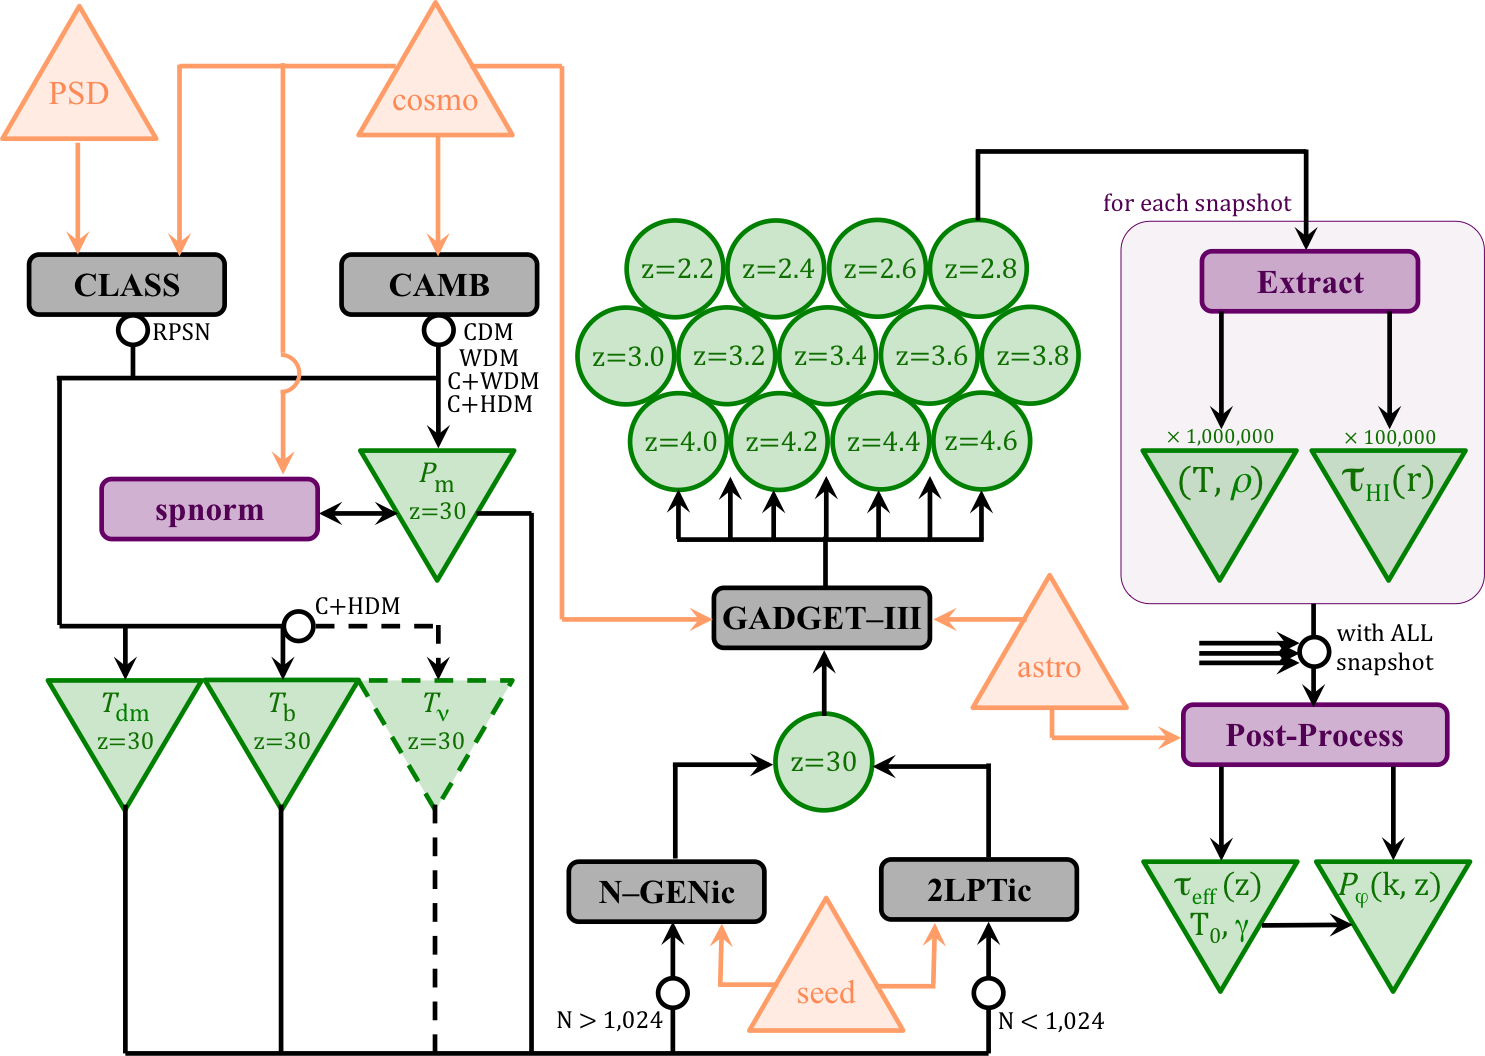
\includegraphics[width=0.85\columnwidth]{Figures/Simu/pipeline.png}
\caption{Schéma des simulations numériques destinée à construire le spectre de puissance Ly-$\alpha$ à partir de paramètres cosmologiques et astrophysique, précisés par l'utilisateur, en triangles oranges. Les triangles inversés verts correspondent aux sorties des logiciels. Les cercles verts sont des fichiers sortie (snapshot) de \textsf{Gadget-3}. Les boîtes en gris/noir sont les logiciels en accès-libre. Les encadrés violets sont des scripts internes à la collaboration SDSS/BOSS.}
\label{fig:pipeline}
\end{center}
\end{figure}

Le spectre de puissance de flux transmit dans la forêt Ly-$\alpha$ ($P_\varphi$) attendu est construit à l'aide de simulations numériques. $P_\varphi (k, z)$ est évalué aux 12 bins en redshift correspondant aux donnés, plus $z=4.6$ puisqu'il est envisagé de rajouter ce bin avec la DR14 de eBOSS. Il est construit en calculant la transformé de Fourier des fluctuations de baryons moyenné sur $10^5$ lignes-de-visées tirées aléatoirement dans une boîte de $100~h^{-1}\mathrm{Mpc}$ de côté\footnote{avec conditions périodiques aux bords} comptant $3072^3$ particules de baryon, $3072^3$ particules matière noire et $3072^3$ neutrinos. Les positions et vitesses de chaque particules sont calculées par \textsf{Gadget-3} (GAlaxies with Dark matter and Gas intEracT), un code écrit en ANSI C massivement parallélisé\footnote{pour l'étude sur la masse des neutrinos, le code a été tourné sur plus de $8000$ coeurs du calculateur \textsf{Curie} du TGCC.}, developé par \cite{Springel2001, Springel2005}.  \\

\textsf{Gedget-3} emploie l'interface standardisé de transmission de message (\texttt{MPI}) ainsi que plusieurs librairies à accès libre (\texttt{GSL}\footnote{\url{http://www.gnu.org/software/gsl/}}, \texttt{FFTW}\footnote{\url{http://www.fftw.org/}}). Les interactions gravitationnelles sont calculées à travers une expansion multipolaire hiérarchique en utilisant la méthode classique du problème à $N$-corps, tandis que l'hydrodynamique est résolue en utilisant une description SPH (smoothed particle hydrodynamics). Le code résoud le problème $N$-corps pour les composantes décrites par un fluide sans collisions (matière noire et neutrinos) en même temps que le SPH pour la composante baryonique, chaque composante étant couplée aux autres ainsi qu'à la métrique espace-temps, en expansion uniforme et isotrope. Le code modélise également certains mécanismes de contre-réaction entre petites et grandes échelles, la formation d'étoiles, le réchauffement/refroidissement radiatif du MIG \textit{etc}. \\

En raison des vitesses très élevées des neutrinos, initier les simulations cosmologiques à $z_{\mathrm{ic}}=100$ leur confèrerait un bruit de Poisson trop élevé. Afin de réduire cette nuisance, les simulations sont initiées à $z_{\mathrm{ic}}=30$, puisque la vitesse des neutrinos décroit linéairement avec le facteur d'échelle $a$. Au-delà de ce redshift de départ, une description Lagrangienne au second ordre des perturbation est suffisante pour résoudre les positions et vitesses des particules \citep{Crocce2006}. Résoudre exactement les intéractions serait coûteux et inoptimal, puisque le spectre de puissance de matière seul suffit à décrire le système baryon + matière noire + neutrinos. Le spectre de puissance de matière est calculé avec le logiciel \textsf{CAMB} \citep{Lewis2011} ou \textsf{CLASS} \citep{CLASS}, et les conditions initiales pour la prise-en-main de \textsf{Gadget-3} s'effectue grâce au code \textsf{2LPTic} ou \textsf{N-GENic}, en fonction du nombre de particules dans la boîte de simulation. Le schéma des simulations est illustré par étapes dans la figure \ref{fig:pipeline}. La figure \ref{fig:visu} montre la distribution du gaz baryonique à $z=2.5$, dans une simulation de plus petite taille ($2 \times 768^3$ particules dans un volume de $(25~h^{-1}\mathrm{Mpc})^3$) destinée à la résolution des petites échelles. La température (densité, respectivement) du gaz est représenté par la couleur (contraste). Les images sont réalisées avec le logiciel \textsf{Splotch}\footnote{\url{http://www.mpa-garching.mpg.de/~kdolag/Splotch}}. On distingue le réseau filamentaire sur lequel s'organise la matière aux très grandes échelles, conformes aux observations des relevés des grandes structures (2dF, SDSS, DES). Dans chacun des encadrés, la matière noire est constituée de neutrinos stériles de masse décroissante (dans le sens horaire en partant du haut à gauche). Comme prédit par la théorie linéaire des perturbations (voir figure \ref{fig:pm}), plus la masse de la particule matière noire est légère, plus la distance caractéristique qu'elle parcours est élevée, empêchant l'effondrement gravitationnelle aux échelles en-dessous de cette distance caractéristique. \\

\begin{figure}
\begin{center}
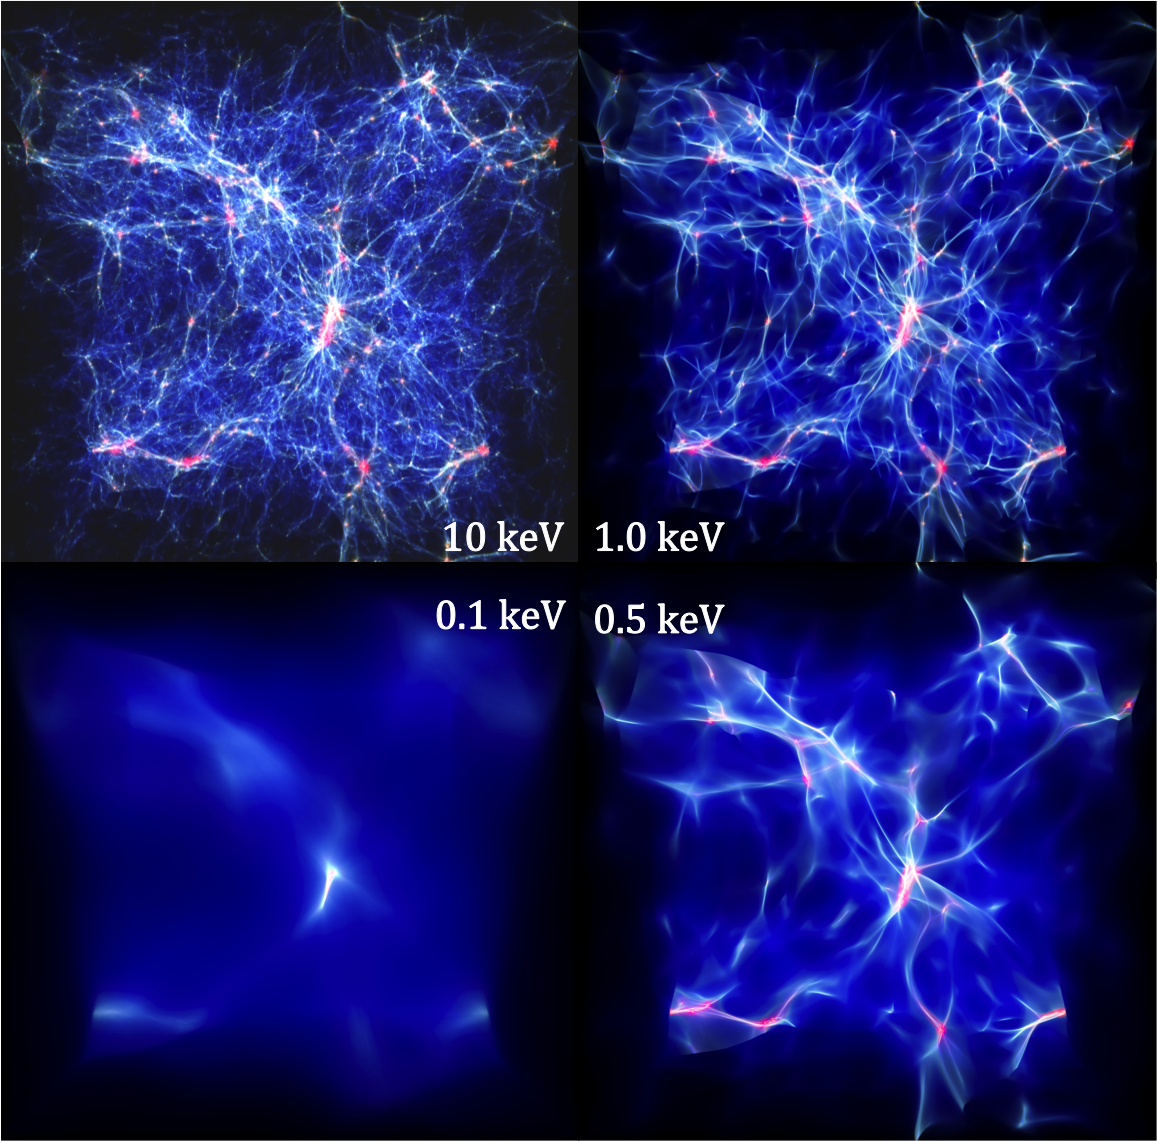
\includegraphics[width=0.85\columnwidth]{Figures/Visu/CWH.png}
\caption{Visualisation de la température (couleur) et densité (contraste) du gaz baryonique dans les simulations hydrodynamiques, avec une masse de la particule matière noire explicite dans le coin de chaque encadré.}
\label{fig:visu}
\end{center}
\end{figure}

Afin de quantifier l'impact de la masse des neutrinos sur le spectre de puissance Ly-$\alpha$, il est nécessaire de tourner des simulations numériques dans plusieurs configurations. Il est également nécessaire de modifier une liste de paramètres cosmologiques et astrophysiques pour distinguer l'effet de la masse des neutrinos d'éventuelles dégénérescences avec ceux-ci, notamment: \\
\begin{itemize}
\item[$\bullet$] la densité énergétique de la matière $\Omega_m$; \\
\item[$\bullet$] l'écart-type des fluctuations de matière à $8~\mathrm{Mpc}$, $\sigma_8$; \\
\item[$\bullet$] le taux d'expansion $H_0 = \left. \cfrac{\dot{a}}{a} \right\vert_{a=1}$; et \\
\item[$\bullet$] l'indice spectral du spectre de puissance des fluctuations primoridales $n_s = \cfrac{d \mathcal{P}}{d \log k}$ \\
\end{itemize}

où le spectre de puissance initial s'écrit \\
\begin{equation}
\mathcal{P} (k) = \mathcal{A}~\left( \frac{k}{k_\star}\right)^{n_s}
\end{equation} \\ et décrit les fluctuations du champs gravitationnel à très grand redshift. $k_\star = 0.05~\mathrm{Mpc}^{-1}$ est l'échelle de pivot du CMB. Les spectre de puissance de chaque espèce (neutrino, matière noire, baryons, photons) y est relié par \\
\begin{equation}
P_i (k,z) = \mathcal{P} (k) \times T^2_i (k) \times \mathcal{D}_i^2 (z)
\end{equation} \\ où $\mathcal{D}_i$ est la fonction d'accroissement des structures et $T_i$ la fonction de transfert, qui est calculé dans \textsf{CAMB}. L'amplitude $\mathcal{A}$ est reliée à $\sigma_8$ puisque ce dernier est une intégrale du spectre de puissance jusqu'à l'échelle $8~\mathrm{Mpc}$. Leur effet sur le spectre de puissance Ly-$\alpha$ est illustré sur la figure \ref{fig:cosmo}. \\

\begin{figure}
\begin{center}
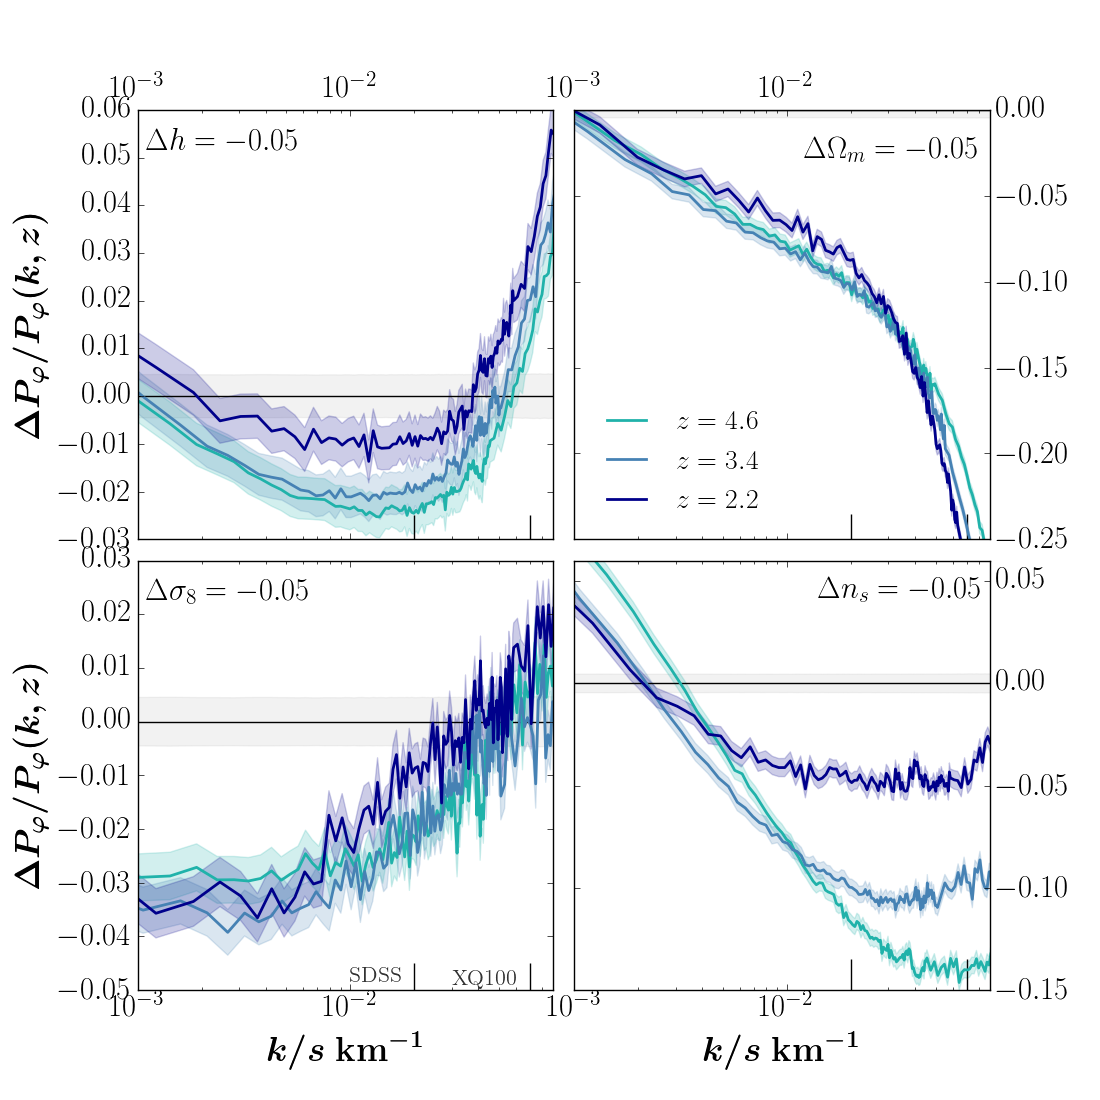
\includegraphics[width=0.85\columnwidth]{Figures/Cosmo_Pf.png}
\caption{Différence relative du spectre de puissance du flux Ly-$\alpha$ par rapport au modèle central (sans neutrinos, en trait noir) à 3 redshifts, pour les 4 paramètres cosmologiques libres des simulations. L'épaisseur quantifie l'incertitude sur $P_\varphi$ dans les simulations numériques.}
\label{fig:cosmo}
\end{center}
\end{figure}

L'état thermodynamique du milieu intergalactique influence également la profondeur optique et donc le spectre de puissance Ly-$\alpha$. Afin de distinguer l'effet de la masse des neutrinos des effets de lissage dû à la température du MIG
\begin{equation}
T(\delta, z) = T_0 (z) \times \left( 1 + \delta \right)^{\gamma(z) - 1}
\end{equation} et de la dépendance en redshift de la profondeur optique effective
\begin{equation}
\tau_\mathrm{eff} (z) = A^\tau \times \left( 1 + z \right)^{\eta^\tau}
\end{equation} les simulations numériques tournent sur des valeurs fluctuantes de \\
\begin{itemize}
\item[$\bullet$] la température moyenne du MIG à $z=3$, $T(\delta=0,z=3)$; \\
\item[$\bullet$] l'indice de température à $z=3$, $\gamma(z=3)$; \\
\item[$\bullet$] le redshift de ré-ionization $z_\star$; \\
\item[$\bullet$] la profondeur optique effective à $z=3$, $A^\tau (z=3)$; et \\
\item[$\bullet$] l'indice de la profondeur optique effective à $z=3$, $\eta^\tau (z=3)$. \\
\end{itemize} Le spectre de puissance Ly-$\alpha$ à un set de paramètres
\begin{equation}
\vec{x} = \left( m_\nu^\mathrm{eff}, h, \Omega_m, \sigma_8, n_s, z_\star, T_0^{z=3}, \gamma^{z=3}, A^\tau, \eta^\tau \right)^\mathrm{T}
\end{equation} est évalué à l'ordre 2 d'une expansion de Taylor autour d'un modèle central $\vec{x}_0$, 
\begin{align*}
f(\vec{x}_0 + \Delta \vec{x}) &\simeq f(\vec{x}_0)\\
&+ \sum_i \left. \cfrac{\partial f}{\partial x_i} \right\vert_{\vec{x} = \vec{x}_0} \Delta x_i \\
&+ \frac{1}{2}  \sum_{i} \sum_{j}  \left. \cfrac{\partial^2 f}{\partial x_i \partial x_j} \right\vert_{\vec{x} = \vec{x}_0} \Delta x_i \Delta x_j \\
&+ \mathcal{O} \left( \left\vert \Delta \vec{x} \right\vert^3 \right) 
\end{align*} où les valeurs centrales de chaque paramètre libre et leur écart où sont évaluées les dérivées sont répertoriées dans le tableau \ref{tab:parametres}. \\

\begin{table}
\begin{center}
\begin{tabular}{ccccl}
\hline \\[-10pt]
\hline \\[-10pt]
\textbf{paramètre} &  & $\pmb{x_{0,i}}$ & & $\pmb{\Delta x_i}$ \\[2pt]
\hline \\[-10pt]
\hline \\[-10pt]
\multicolumn{5}{l}{\textbf{paramètres cosmologiques}} \\[2pt]
$h$ & $=$ & $0.675$ & $\pm$ & $0.05$  \\[2pt]
$\Omega_m$ & $=$ & $0.31$ & $\pm$ & $0.05$  \\[2pt]
$\sigma_8$ & $=$ & $0.83$ & $\pm$ & $0.05$  \\[2pt]
$n_s$ & $=$ & $0.96$ & $\pm$ & $0.05$  \\[2pt]
\hline \\[-10pt]
\multicolumn{5}{l}{\textbf{masse des neutrinos}} \\[2pt]
$\sum m_\nu / \mathrm{eV}$ & $=$ & $0.0$ & $+$ & $0.4,0.8$  \\[2pt]
$\mathrm{keV}/m_x$ & $=$ & $0.0$ & $+$ & $0.2,0.4$  \\[2pt]
\hline \\[-10pt]
\multicolumn{5}{l}{\textbf{paramètres astrophysiques}} \\[2pt]
$T^{z=3}_0/10^3\mathrm{K}$ & $=$ & $14.0$ & $\pm$ & $7.0$  \\[2pt]
$\gamma^{z=3}$ & $=$ & $1.3$ & $\pm$ & $0.3$  \\[2pt]
$A^\tau / 10^{-3}$ & $=$ & $2.5$ & $\pm$ & $2.0$  \\[2pt]
$\eta^\tau$ & $=$ & $3.7$ & $\pm$ & $0.4$  \\[2pt]
$z_\star$ & $=$ & $12.0$ & $\pm$ & $4.0$  \\[2pt]
\hline \\[-10pt]
\end{tabular}
\caption{Valeur centrale et pas des paramètres libres des simulations.}
\label{tab:parametres}
\end{center}
\end{table}

L'avantage de cette méthode est qu'il n'est pas nécessaire d'évaluer le spectre de puissance Ly-$\alpha$ sur une grille de paramètres, ce qui serait trop coûteux pour nos simulations puisque chaque consomme environ $5 \times 10^4$ heures CPU. En effet, pour $N$ paramètres, la méthode de l'expansion de Taylor ne nécessite de ne tourner que un modèle central, $2N$ termes du premier ordre et $N(N-1)/2$ termes du second-ordre puisque l'on fait l'hypothèse que $\partial^2_{x_i, x_j} f = \partial^2_{x_j, x_i} f$. En revanche, la validité de cette méthode nécessite que les variations du spectre de puissance dans cet espace de paramètre suivent une loi distribution quasi-gaussienne, ce qui est vérifié \citep{Borde2014}. La figure \ref{fig:taylor_grid} illustre les $6$ simulations à tourner pour $N=2$.\\

\begin{figure}
\begin{center}
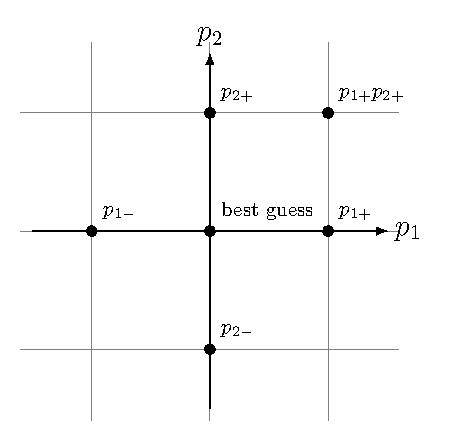
\includegraphics[width=0.5\columnwidth]{Figures/Dari/simulation_grid.pdf}
\caption{Illustration de la grille de Taylor au second ordre en 2 dimensions.}
\label{fig:taylor_grid}
\end{center}
\end{figure}

